\documentclass[a4paper, 12pt, oneside]{Thesis}  % Use the "Thesis" style, based on the ECS Thesis style by Steve Gunn

% \graphicspath{Figures/}  % Location of the graphics files (set up for graphics to be in PDF format)
\usepackage{float}
\usepackage{multirow}
\usepackage{lipsum}
\usepackage{siunitx}
\usepackage{physics}
\usepackage{graphicx}
\usepackage{verbatim}  % Needed for the "comment" environment to make LaTeX comments
\usepackage{vector}  % Allows "\bvec{}" and "\buvec{}" for "blackboard" style bold vectors in maths
\usepackage[square, numbers, comma, sort&compress]{natbib}  % Use the "Natbib" style for the references in the Bibliography

\hypersetup{urlcolor=blue, colorlinks=true}  % Colours hyperlinks in blue, but this can be distracting if there are many links.

%% ------------------ tikz ---------------------------------------
\usepackage{tikz}
\usetikzlibrary{shapes.geometric, arrows,cd}
\tikzstyle{startstop} = [rectangle, rounded corners, minimum width=3cm, minimum height=1cm, text centered, draw=black, fill=white]
\tikzstyle{arrow1}=[ultra thick,->,>=stealth]
\tikzstyle{arrow}=[thick,->,>=stealth]
\tikzset{
  shift left/.style ={commutative diagrams/shift left={#1}},
  shift right/.style={commutative diagrams/shift right={#1}}
}

%%------------------------------------------------------MAIN DOCUMENT------------------------------------------------------
\begin{document}

\frontmatter
\title  {[Wobbling Title]}
\authors  {\texorpdfstring
            {\href{robert.poenaru@drd.unibuc.ro}{Robert Poenaru}}
            {Robert Poenaru}
            }
\addresses  {\groupname\\\deptname\\\univname}  % Do not change this here, instead these must be set in the "Thesis.cls" file, please look through it instead
\date       {\today}
\subject    {}
\keywords   {}

\maketitle
\setstretch{1.3}  % It is better to have smaller font and larger line spacing than the other way round
% Define the page headers using the FancyHdr package and set up for one-sided printing
\fancyhead{}  % Clears all page headers and footers
\rhead{\thepage}  % Sets the right side header to show the page number
\lhead{}  % Clears the left side page header
\pagestyle{fancy}  % Finally, use the "fancy" page style to implement the FancyHdr headers

% The Abstract Page
\addtotoc{Abstract}  % Add the "Abstract" page entry to the Contents
\abstract{
\addtocontents{toc}{\vspace{1em}}  % Add a gap in the Contents, for aesthetics
Nova.

\textbf{Keywords}: \textit{nuclear shape, nuclear deformation, collective parameters, triaxiality, wobbling}.
}
\clearpage

\setstretch{1.3}  % Reset the line-spacing to 1.3 for body text (if it has changed)

% The Acknowledgements page, for thanking everyone
\acknowledgements{
\addtocontents{toc}{\vspace{1em}}  % Add a gap in the Contents, for aesthetics
Nova.

\textbf{Keywords}: Thank you!
}
\clearpage
\tableofcontents
\pagestyle{fancy}  % Return the page headers back to the "fancy" style
%% ----------------------------------------------------------------
\mainmatter	  % Begin normal, numeric (1,2,3...) page numbering

\chapter{Introduction}

Ground-state nuclei possessing spherical or axial symmetry are predominant across the char of nuclides. Near closed shells, the deformation is sufficient that models based on spherical symmetries can be used to describe nuclear properties (e.g., energies, quadrupole moments, and so on). Besides the spherical and axially-symmetric shapes, the existence of triaxial nuclear deformation was theoretically predicted a long time ago \cite{bohr1998nuclear}. The rigid triaxiality of nuclei is defined by the asymmetry parameter $\gamma$, giving rise to a unique behavior concerning the system dynamics. Lately, triaxial nuclei drew a lot of attention within the nuclear physics community, since the description of nuclear properties represents a real challenge from an experimental and also theoretical standpoint. Great progress towards experimental setups being able to perform measurements of high-spin has only been possible after the 2000s. It is worth mentioning that some experiments regarding alpha-$\alpha$ particle reactions induced in heavy nuclei in the early 1960s (e.g., \cite{morinaga1963gamma}) helped to produce a decent amount of data for the rotational in the high-spin region ($\geq 20 \hbar$).

The physics of \emph{high-spin} states has been studied since the early 1950s, with the major breakthrough on the theoretical side made by Bohr and Mottelson \cite{bohr1998nuclear}. The nuclear rotation was described in terms of the rotational degrees of freedom associated with other nuclear degrees of freedom such as particle-vibration, quadrupole-quadrupole, parity, and so on. The spherical shell-model only describes nuclei near the closed shells. On the other side, for the nuclei that lie far from closed shells, a deformed potential must be employed. In the case of even-even nuclei, unique band structures resulting from the vibrations and rotations of the nuclear surface appear in the energy range $0-2\ \text{MeV}$.

Even though triaxiality has an elusive character, two phenomena, i.e., wobbling motion and chiral bands are uniquely attributed to triaxial shapes. Consequently, these two were intensively searched by using advanced techniques. In this work, the focus is given exclusively on the first effect, although it is worth specifying that the current team provides a unified description of both phenomena in their most recent work \cite{raduta2022simultaneous}, which stands out as the first-ever theoretical treatment describing wobbling and chirality on an equal footing.

Quantized wobbling modes were first discovered experimentally in $^{163}$Lu, where the presence of the odd-proton $i_{13/2}$ grants the apparition of multiple rotational bands to appear around the yrast line. This experiment consisted of populating high-spin states with a $^{29}$Si beam interacting with a thin target of $^{139}$La. Later on, other odd-$A$ nuclei were discovered as exhibiting wobbling excitations, and all the experimental findings will be mentioned in the following chapters. The nuclei having a triaxial shape can rotate about any of the principal axes, causing rich collective spectra to emerge. The family of rotational bands is described in terms of vibrational excitations. As a classical analog, nuclear wobbling motion corresponds to the spinning motion of an asymmetric top. The experimental fingerprints for wobbling motion indicate that the energy spectrum behaves as $\sim I(I+1)$ with respect to the angular momentum, there is a clear dominance of electric transitions over the magnetic ones, and the nuclei have large quadrupole moments. All these quantities will be exploited in detail in the coming chapters.

\section{Aim}

The objective of this research is two-fold. On one side, the theoretical description of wobbling motion is treated in detail, starting from the required nuclear models specific to deformed nuclei, and reaching a set of key properties of the phenomenon. Differences between wobbling that occurs in odd- but also even-mass nuclei are depicted since each situation manifests in remarkable ways. Once the general formalism behind this effect is presented, an inventory of all the currently identified nuclei will be made, providing clear explanations for the band structure and also the relevant parameters describing deformation. The complete overview of all existing wobbling nuclei is encapsulated in a unified informative chart, which is in fact one of the unique features of the research, and a first within the literature.

The second objective of this present work is to describe the wobbling mechanism by means of a novel semi-classical approach. Indeed, the important quantities related to collective excitations are properly reproduced by the, i.e., excitation energies, quadrupole moments, transition probabilities, and many more. This model starts from an initial quantal Hamiltonian that is dequantized through a variational method. A set of classical equations of motion that describe triaxial nuclei are obtained, and a classical energy function is granted by the approach. This function is a remarking feature of the developed framework, as this fully analytical expression (containing only classical variables that were obtained via the dequantization) will provide an insight into multiple analyses: energy spectrum, stability of the wobbling motion, critical regions, phase transitions and even possible changes in the wobbling regime. 

Another remarking feature of the current model is the geometrical interpretation of the rotational motion specific to triaxial nuclei, which is described in both a two- and three-dimensional space. Also unique to this research is the introduction of two concepts that are related to the band structures of odd-mass nuclei. These are the Signature Partner Bands and Parity Partner Bands and they can be considered hallmarks of the theory. Lastly, it is worth mentioning that throughout this entire work, a consistent graphical representation is adopted, giving workflow diagrams, schematics, and charts, with the purpose of providing clearer explanations (where possible) of the underlying mechanisms.

\section{Motivation}

Over the years, many theoretical interpretations were suggested for the description of the wobbling motion and its main features. The Triaxial Rotor Model \cite{bohr1998nuclear,davydov1958rotational} and the Particle Rotor Model \cite{hamamoto2002wobbling} are quantal models that are solved exactly in the laboratory frame. Other investigations are based on mean-field theories, such as the Random Phase Approximation \cite{shimizu1995nuclear}, the Angular Momentum Projection \cite{oi2000wobbling}, and also the Collective Hamiltonian \cite{chen2014collective} were adopted.

This research aimed at a semi-classical description of the wobbling phenomenon due to its advantage in keeping close contact with the `classical picture' of the system dynamics. Certainly, working with a set of classical equations of motion is much easier than having to deal with quantum mechanical objects that do not have a clear one-to-one correspondence with classical mechanics. It will be shown that the rotational motion of a triaxial nucleus can be approximated quite well with that of a rigid rotator, meaning that the energy spectrum could be accurately described through quantities that have concise physical meaning (i.e., moments of inertia, angular momentum, angular frequency). Moreover, the analytical spectrum that is achieved by solving the equations for an odd-mass nucleus is indeed remarkable, since it will be described by separated degrees of freedom associated with an even-even core and a valence nucleon that interacts with the core. The variational method that is employed proves to be an efficient tool in accurately depicting the energy spectra and transition probabilities of several odd-$A$ nuclei within the $A=160$ mass region.

The lack of studies of geometrical treatments for the wobbling motion encouraged the team to pursue such an analysis. A two-dimensional evaluation shows if regions of stability exist, meaning that one can identify the energies at which the total angular momentum exhibits stable precessional motion. Taking the formalism a step further, the wobbling motion is explored within the space generated by the three components of the total angular momentum. The two constants of motion, i.e., the total energy and the total spin are graphically represented in the same picture, and their intersection signifies the allowed trajectories that the angular momentum precesses around. Each trajectory corresponds to a particular set of spin and energies, meaning that the entire spectrum of a wobbling nucleus can be interpreted. Using the classical view of the angular momentum and the total energy for a triaxial ellipsoid represents the onset of a fully unified description of nuclear deformation. Moreover, this phenomenological and semi-classical model gives results that are on par with fully microscopic or quantal descriptions (much more complex), making it a successful tool in describing collective phenomena.

\section{Thesis Structure}

This thesis is structured in the following way. Chapter \ref{chapter-2-theoretical-aspects} begins with the study of the nuclear surface using the expansion of the radius $R$ in terms of collective coordinates and spherical harmonics. The multipole modes are presented and a focus on the quadrupole $\lambda=2$ excitation mode is considered. This is the main vibrational mode causing triaxial deformation of the nucleonic matter. Within the approximation of the nuclear surface, the deformation parameters $\beta_2$ and $\gamma$ are introduced, which give a direct insight with respect to the degree of elongation and asymmetry between the ellipsoid axes. Furthermore, the theoretical models necessary to describe the deformed nuclei are sketched in Section \ref{section-nuclear-models} within the same chapter. Starting with the Spherical Shell-Model, a step-by-step procedure is considered and more complete models such as the Deformed Shell, Nilsson, or even the Collective model are constructed. The last section of the chapter (Section \ref{section-triaxial-signatures}) presents two fingerprints of triaxiality, i.e., chiral motion and wobbling motion. Concerning the chiral bands, some experimental data are presented, and nucleonic configurations that lead to the apparition of chiral motion are geometrically represented. 

Wobbling motion, which is the `core' topic of this research is treated in Chapter \ref{chapter-3}, where its physical meaning is given. The difference between wobbling in odd- and even-mass nuclei is provided, and the two wobbling regimes that emerge in the odd-$A$ nuclei are portrayed. A quantal approximation made by Frauendorf in Ref. \cite{frauendorf2014transverse} shows that based on the alignment of the valence nucleon and the even-even core, two possible wobbling modes occur: transverse and longitudinal. The modes are properly outlined giving geometrical interpretations and showing key differences between the involved quantities. Using an approximation for an initial Hamiltonian of a rigid triaxial rotor, a proper analytical expression is obtained for the even-$A$ nuclei. The energy spectrum is defined as the sum between a quadratic term in angular momentum and a harmonic-like term. With this formula, the experimental wobbling bands in $^{130}$Ba are successfully reproduced, together with the transition probabilities of the collective states. Also in Chapter \ref{chapter-3}, all known experimental findings concerning wobbling excitations are specified, finishing with a chart that contains relevant parameters for each nucleus in particular. 

In Chapter \ref{chapter-4-aw1-formalism}, the theoretical formalism for describing odd-mass nuclei is employed. This semi-classical model starts from a Time-Dependent Variational Equation applied on a Particle-Rotor Hamiltonian. From this, a classical energy function is attained, and it is used two describe the excited spectra of triaxial nuclei. The energy spectrum is parametrized in terms of the moments of inertia, the triaxiality $\gamma$, and the interaction strength between the core and the odd-particle. These five free parameters are determined by fitting the excitation energies of $^{161,163,165,167}$Lu to the experimental data. Other quantities such as transition probabilities, alignments, and dynamical moments of inertia are calculated for each isotope with the obtained parameter set. A key feature of the approach depicted in Chapter \ref{chapter-4-aw1-formalism} is the renormalization of the wobbling band structure in terms of Signature Partner Bands. The method is compared with a previous description that adopted a different mechanism for obtaining wobbling excitations.

A novel method for studying wobbling motion in odd-mass nuclei is discussed in Chapter \ref{chapter-5-novel}, starting from the considerations made in the previous chapter. Herein, through the concept of Parity Partner Bands, it is shown that the wave-function describing the triaxial nuclei admits states of both positive and negative parity, which makes it possible to use an even simpler analytical spectrum of $^{163}$Lu. Another fitting method is employed for the entire spectrum, including a rotational band that previously was treated separately. Consequently, a set of results that are very close to the real values is obtained. For a classical description, these results are quite impressive, as they are the first within the literature that achieve deviations under $100\ \text{keV}$ across the entire spectrum of $^{163}$Lu. Identification of phase transitions, where the nucleus could change its rotational mode, but also regions where rotational motion is unstable, are obtained through graphical representations within a space generated by dequantized variables that describe the rotational degrees of freedom for the particle + rotor system. 

Chapter \ref{extra-chapter-new-boson} presents a specialized description of wobbling motion in odd-mass nuclei, based on a recent case study conducted by the team on $^{135}$Pr. Utilizing a boson representation of angular momentum components and the initial Hamiltonian yielded accurate results for both the energy spectrum and transition probabilities. The numerical implementation of this approach involved fitting experimental data and utilizing a set of well-established trigonometric functions - specifically, the Jacobi Elliptic Functions. These functions provide valuable insights into the potential energy, wobbling frequency, and stability of odd-mass triaxial nuclei.

In Chapter \ref{chapter-8-conclusions}, concluding remarks are provided that summarize the key findings and contributions of this entire work. It should be noted that several chapters also contain their own set of conclusions, which offer more detailed insights into the specific topics covered within those chapters. % Introduction
\chapter{Deformed Nuclei}

\section{Nuclear deformation}

Most of the nuclei across the nuclide chart are spherical or symmetric in their ground state. Moreover, for the axially symmetric nuclei (i.e, either \emph{oblate} or \emph{prolate}), there is a prolate over oblate dominance.
% \begin{figure}[ht]
%     \centering
%     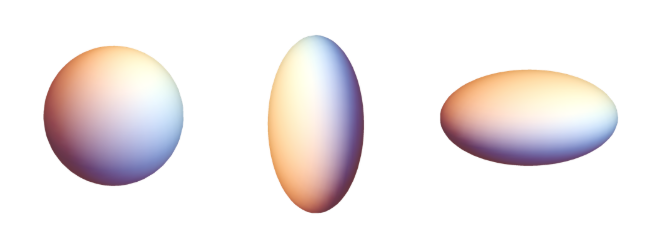
\includegraphics[scale=0.3]{Chapters/Figures/nuclear_shapes.png}
%     \caption{Nuclear Shapes.}
%     \label{nuclear_shapes}
% \end{figure}

The spherical shell model only describes nuclei near the closed shells. On the other side, for the nuclei that lie far from closed shells, a deformed potential must be employed. 
\par In the case of even-even nuclei, unique band structures resulting from the vibrations and rotations of the nuclear surface (as proposed by Bohr and Mottelson \cite{bohr1998nuclear} in the \emph{Geometric Collective Model} - GCM) appear in the energy range 0-2 MeV.

Within the GCM, the nucleus is described as a classical charged liquid drop. For the low-lying energy spectrum, usually, the compression of nuclear matter and the nuclear skin thickness are neglected. This results in the final picture of a liquid drop with a constant nuclear density and a sharp surface \cite{greiner1996nuclear}.

\subsection{Collective coordinates}

The nuclear surface can be described via an expansion of the spherical harmonic functions with some time-dependent parameters as \emph{expansion coefficients}. The expression of the nuclear shape is shown below \cite{greiner1996nuclear}:
\begin{align}
    R(\theta,\varphi,t)=R_0\left(1+\sum_{\lambda=0}^\infty\sum_{-\lambda}^\lambda\alpha_{\lambda\mu}(t)Y_\lambda^\nu(\theta,\varphi)\right)\ .
    \label{nuclear-shape}
\end{align}

In \ref{nuclear-shape}, $R$ denotes the nuclear radius as a function of the spherical coordinates $\theta,\varphi)$ expressing the direction, and the time $t$, while $R_0$ is the radius of the spherical nucleus when all the expansion coefficients vanish. It is worth mentioning that the expansion coefficients $\alpha_{\lambda\mu}$ act as \emph{collective coordinates} since the time-dependent amplitudes describe the vibrations of the nuclear surface.

\subsection{Nuclear radius under rotation}

To get a grasp at the physical meaning behind the deformation parameters that are used to describe the nuclear surface, it is instructive to see what happens when the system undergoes a rotation transformation.

The function $R(\theta,\varphi)$ describes the original (non-rotated) nuclear shape. Rotating the system will result in the change of the angular coordinates $(\theta,\varphi)$ to $(\theta',\varphi')$, which will correspond to a new function $R'(\theta',\varphi')$. Moreover, both nuclear surfaces (i.e., the non-rotated and the rotated one) must hold the equality:
\begin{align}
    R'(\theta',\varphi')=R(\theta,\varphi)
\end{align}

The rotational invariance of $R$ employs that $R'(\theta,\varphi)$ must have the same functional form, but the expansion coefficients $\alpha_{\lambda\mu}$ must be rotated, meaning:
\begin{align}
    \sum_{\lambda\mu}\alpha_{\lambda\mu}'Y'_{\lambda\mu}(
        \theta,\varphi)=\sum_{\lambda\mu}\alpha_{\lambda\mu}Y_{\lambda\mu}(
            \theta,\varphi)\ . \label{nuclear_surface_equality}
\end{align}

Note that in Eq. \ref{nuclear_surface_equality}, the spherical harmonics $Y'_{\lambda\mu}$ are obtained via the usual rotation matrices. Finally, the invariance of Eq. \ref{nuclear-shape} is achieved if the set of parameters $\alpha_{\lambda\mu}$ transform similarly to a \emph{spherical tensor with angular momentum} $\lambda$ \cite{ring2004nuclear}, that is:
\begin{align}
    \alpha_{\lambda\mu}'=\sum_{\mu'}\mathcal{D}^{(\lambda)}_{\mu\mu'}\alpha_{\lambda\mu'}\ .
\end{align}

Besides the spherical tensor character, the collective coordinates also have the following properties (emerging from Eq. \ref{nuclear-shape}):
\begin{itemize}
    \item Complex Conjugation.
    \begin{align}
        Y^*_{\lambda\mu}(\theta,\varphi)&=(-1)^{\mu}Y_{\lambda-\mu}(\theta,\varphi), \\
        \alpha^*_{\lambda\mu}&=(-1)^\mu\alpha_{\lambda-\mu}\ .
    \end{align}
    \item Parity - the coordinates $\alpha_{\lambda\mu}$ must undergo the same change of sign under a parity transformation as the spherical harmonics, in order to keep the invariance of the nuclear surface.
    \begin{align}
        (r,\theta,\varphi) &\xrightarrow[P]{}     (r,\pi-\theta,\pi+\varphi)\ \nonumber, \\
        Y_{\lambda\mu}(\theta,\varphi) &\xrightarrow[P]{} Y_{\lambda\mu}(\pi-\theta,\pi+\varphi)=(-1)^\lambda Y_{\lambda\mu}(\theta,\varphi)\ .\nonumber
    \end{align}
    Therefore, the parity of the expansion coefficients are:
    \begin{align}
        \pi(\alpha_{\lambda\mu})=(-1)^\lambda\ .
    \end{align}
\end{itemize}

\subsection{Multipole deformations}

In the expansion of the nuclear surface defined by Eq. 
\ref{nuclear-shape}, the different values for $\lambda$ will determine different effects regarding the physical aspects of the nucleus. As such, the first values of $\lambda$ will be examined in terms of the physical meaning.

\begin{description}
    \item[Monopole mode] This corresponds to the first value of $\lambda=0$. This is the simplest mode of \emph{deformation} of a nuclear surface. Within this approximation, the spherical harmonic $Y_0^0$ is constant, which would imply that any non-vanishing values for $\alpha_{00}$ will correspond to the change in radius of the nucleus. This kind of excitation is also called \emph{breathing mode} of the nucleus \cite{greiner1996nuclear,bohr1998nuclear}. The energy required for this kind of excitation mode is very large, since it implies a compression of the nuclear matter. As a result, this mode is irrelevant in the low-lying excited spectra of atomic nuclei.
    \item[Dipole mode] Corresponds to $\lambda=1$. In reality, this type of mode does not manifest itself as a deformation of the nucleus, but rather as a shift of the nuclear center of mass. In the lowest order $\lambda=1$, the shift is in fact a translation of the entire nucleus, and it does not represent an actual nuclear excitation.
    \item[Quadrupole mode] Excited modes that correspond to $\lambda=2$. These are the most important collective excitations that take place inside the nucleus. The loss of axial symmetry, triaxial deformations, and other shape-specific transitions that happen within the nucleus are mostly described (and very accurately) via the quadrupole effects.
    \item[Octupole mode] This corresponds to the next increasing value of $\lambda=3$, representing the main asymmetric excitations of a nucleus with states of negative-parity. The specific shape of a nuclear system governed by octuple deformations is similar to that of a pear.
    \item[Hexadecupole deformations] Excitations which correspond to $\lambda=4$. Within the nuclear theory, this is considered the highest angular momentum which can still provide relevant information for the nuclear phenomena that are studied. Currently, there is no clear evidence for pure excitations with hexadecupole nature, however, these excitations seem to have a major role in the admixture to quadrupole excitations for the ground-state shape of heavy nuclei \cite{greiner1996nuclear}.
\end{description}
The multipole deformations for the cases $\lambda=1,2,3$ and $\lambda=4$ discussed above are pictorially shown in Fig. \ref{multipole-deformations}.
Excitations with higher angular momentum than the mentioned ones have practically no application within the study of atomic nuclei. Moreover, one can also see that there is an intrinsic limitation on the maximal value of $\lambda$, which dictates the smallness of the individual bumps of the surface (see Fig. \ref{multipole-deformations}). These bumps are described by the spherical harmonics $Y_\lambda^\mu$, and they decrease in size with increasing values of $\lambda$, but with the physical limitation given by the size of the nucleon diameter.

\begin{figure}
    \centering
    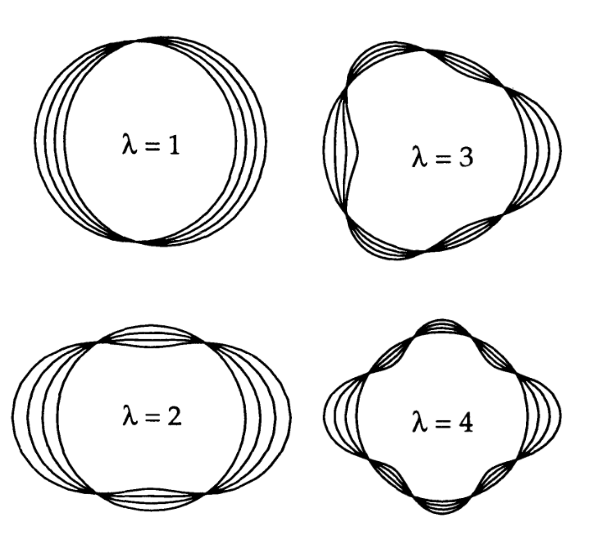
\includegraphics[scale=0.3]{Chapters/Figures/nuclearDeformation.png}
    \caption{Graphical representation for the first few modes of excitations of the nuclear surface. The figure is taken from Ref. \cite{greiner1996nuclear}.}
    \label{multipole-deformations}
\end{figure}

\subsection{Quadrupole Deformation}

One of the most important excitation modes (vibrational degrees of freedom) is the quadrupole deformation, corresponding to $\lambda=2$. In the case of pure quadrupole deformation, the nuclear surface will be given by the following expression:
\begin{align}
    R(\theta,\varphi)=R\left(1+\sum_\mu\alpha_{2\mu}Y_2^\mu(\theta,\varphi)\right)\ . \label{quadrupole-surface}
\end{align}

From this expression, the term $\alpha_{00}$ is of second order in $\alpha_{2\mu}$ and it can be neglected further on. This term also reflects the conservation of volume \cite{greiner1996nuclear,ring2004nuclear}. The real and independent degrees of freedom from the above expression are: $\alpha_{20}$, the real and imaginary parts of $\alpha_{21}$, and the real and imaginary parts of $\alpha_{22}$, respectively.

More insight with regards to the quadrupole shape of the nucleus can be achieved if one expresses $R$ in terms of cartesian coordinates. The spherical harmonics will attain a new form, depending on the cartesian components of the unit vector pointing in a direction defined by $(\theta,\varphi)$:
\begin{align}
    \xi=\sin\theta\cos\varphi\ ,\ \eta=\sin\theta\sin\varphi\ ,\ \zeta=\cos\theta\ ,
\end{align}
with the condition $\xi^2+\eta^2+\zeta^2=1$. With the expressions of the spherical harmonics as functions of $(\xi,\eta,\zeta)$, the nuclear radius will change accordingly (cartesian expression $R=R(\xi,\eta,\zeta)$). A relationship between the cartesian components and the spherical ones for the deformation can be also obtained if one writes all coefficients $\alpha_{2\mu}$ as functions of $\alpha_{ij}$ (with $i,j=\xi,\eta,\zeta$). Since the cartesian deformations can be regarded as closely related to a stretch/contraction of the nucleus in a given direction, a first interpretation of the physical meaning behind the parameters $\alpha_{2\mu}$ can be established:
\begin{itemize}
    \item $\alpha_{20}$: describes the stretching of the $z$ axis with respect to the $y$ and $x$ axes.
    \item $\alpha_{2-2}$ and $\alpha_{22}$: give the relative length of the $x$ axis compared to the $y$ axis. Moreover, it also gives the oblique deformation in the $x-y$ plane.
    \item $\alpha_{2-1}$ and $\alpha_{21}$: describe an oblique deformation, but with respect to the $z$ axis.
\end{itemize}

With the set of parameters defined above, the shape and orientation of the nucleus can have arbitrary values (the coefficients $\alpha_{2\mu}$ are mixing the shape and orientation), thus making the parametrization somewhat problematic. In order to fix that, the geometry can be changed if one considers the \emph{principal axis system} (the PA reference system is a coordinate system in which the moments of inertia associated with the nucleus are diagonal). 
When using this reference frame, the number of parameters is still unchanged, however their physical significance becomes clearer. By denoting the new coordinate system with primed letters, nuclear radius will be described as a function $R=R(\xi',\eta',\zeta')$, with the conditions that $\alpha'_{ij}=0\ ,\ i\neq j$. The condition will further imply that the newly expressed parameters ($\alpha'_{2\mu}$) have the following form:
\begin{align}
    \alpha'_{2 \pm 1}&=0\ , \nonumber \\
    \alpha'_{2 \pm 2}&\equiv a_2\ , \nonumber \\
    \alpha'_{20}&\equiv a_0\ . 
\end{align}
, where the conveniently denoted terms $a_2$ and $a_0$ are some functions that depend on the cartesian components $\alpha_{\xi,\xi}\ ,\ \alpha_{\eta,\eta}\ ,\ \alpha_{\zeta,\zeta}$. From this set of equations the physical significance of the five real and independent parameters is clearer:
\begin{itemize}
    \item $a_0$ is indicating the stretch of $z'$ axis w.r.t. the $x'$ and $y'$ axes.
    \item $a_2$ is indicating the asymmetry between the lengths of $x'$ and $y'$ axes respectively.
    \item the Three \emph{Euler angles} $\mathbf{\theta}=(\theta_1,\theta_2,\theta_3)$. These angles will determine the orientation of the PA system $(x',y',z')$ with respect to the laboratory-fixed frame $(x,y,z)$.
\end{itemize}

One can now clearly see the advantage of working within the PA system: rotation and shape vibration degrees of freedom can be completely separated. A change in the Euler angles will result in a pure rotation of the nucleus (without changing its shape), while a change in shape will be affected exclusively by the $a_0$ and $a_2$ parameters. If $a_2=0$, then the nucleus has a shape with axial symmetry around the $z$ axis (equal axis lengths along the $x$ and $y$ directions).

Another way of describing the excitations of quadrupole type is to adopt the parameters introduced by A. Bohr \cite{bohr1954rotational}. These two parameters can be viewed as a set of polar coordinates in the space generated by $(a_0,a_2)$ and they are defined as:
\begin{align}
    a_0&=\beta_2\cos\gamma\ , \nonumber \\
    a_2&=\frac{1}{\sqrt{2}}\beta_2\sin\gamma\ , \label{bohr-deformation-params}
\end{align}
where the numeric factor $\frac{1}{2}$ was added such that the following relation holds true:
\begin{align}
    \sum_\mu\left|\alpha_{2\mu}\right|^2=\sum_\mu\left|\alpha'_{2\mu}\right|^2=a_0^2+2a_2^2=\beta_2^2\ .
    \label{quadrupole-param-sum}
\end{align}
It is worth mentioning that the Eq. \ref{quadrupole-param-sum} is rotationally invariant, having the same value in the laboratory and the principal axes systems.

Now that the shape of the nucleus (i.e., the nuclear surface radius $R$) can be described consistently with via the parameters defined in Eq. \ref{bohr-deformation-params}, one can calculate the stretching of the nuclear radius along any of the directions is given in terms of $(\beta,\gamma)$ as follows:
\begin{align}
    \delta R_k=\sqrt{\frac{5}{4\pi}}\beta\cos(\gamma-\frac{2\pi k}{3})\ .
\end{align}

\subsubsection{Axial quadrupole deformations}

Using this set of new coordinates, the expression of the nuclear radius for axially quadrupole-deformed nuclei is given as:
\begin{align}
    R(\theta,\varphi)=R_0\left(1+\beta_2 Y_2^0(\theta,\varphi)\right)\ . \label{quadrupole-radius}
\end{align}

In Eq. \ref{quadrupole-radius}, the parameter $\beta_2$ is called the \emph{quadrupole deformation parameter}, and its value dictates wether the nucleus is \emph{oblate} - $\beta_2<0$ (i.e., a flattened sphere), \emph{prolate} - $\beta_2>0$ (i.e., elongated sphere, like a rugby ball), or \emph{spherical} - $\beta_2$.  The nuclear shapes that are characterized only by $\beta_2$ (i.e., $\gamma=0$) have shapes that correspond to spheroids. These shapes are axially symmetric, meaning that they only have one deformed axis. For the spherical case $\beta_2=0$, all three axes have the same lengths, meaning that the shape of the nucleus is in fact a sphere.

For the axially-symmetric quadrupole deformations, the parameter $\beta_2$ can be related to the axes of the spheroid via the formula \cite{greiner1996nuclear}:
\begin{align}
    \delta R_k=\sqrt{\frac{5}{4\pi}}\beta_2\cos\left(\gamma-\frac{2\pi k}{3}\right)\ ,
\end{align}
with $k=1,2,3$ indices that correspond to each of the three principal axes $x'$, $y'$, and $z'$, respectively. The stretching of the nuclear axis in a particular direction (denoted by $k$ in the above formula) varies according to the change in $\gamma$, for a fixed value of $\beta_2$.

\begin{figure}
    \centering
    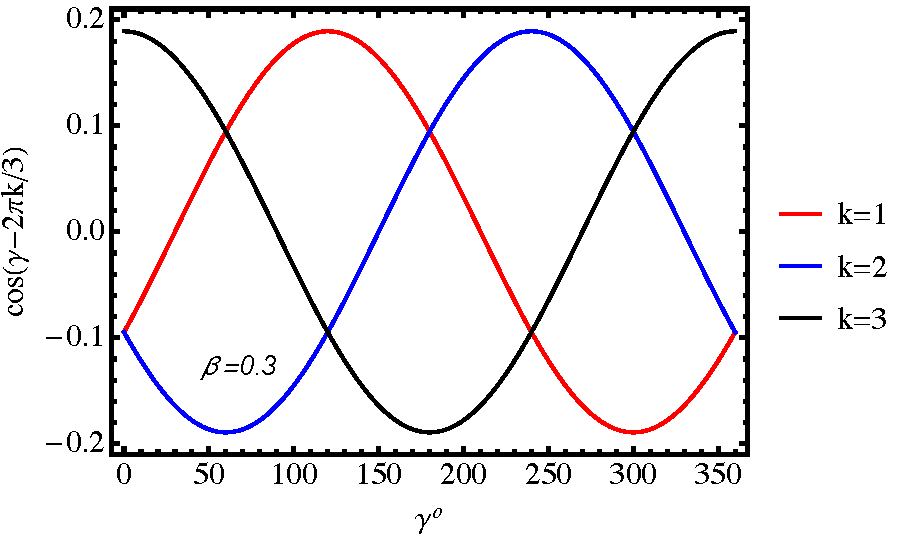
\includegraphics[scale=0.65]{Chapters/Figures/nuclear-radius-elongation.pdf}
    \caption{A graphical representation with the stretching of the nuclear axis $\delta R_k$ for $k=1,2,3$, corresponding to the increase in axis lengths along the $x$, $y$, and the $z$ directions, respectively. The representation used an arbitrary value for the quadrupole deformation $\beta_2=0.3$. Figure was reproduced according to the calculations done in \cite{greiner1996nuclear}.}
    \label{nuclear-radius-elongation}
\end{figure}

Taking a look at Fig. \ref{nuclear-radius-elongation}, one can see the variations of the three axes with $\gamma$. When $\gamma=0^\circ$ the nucleus is elongated along the $z'$ axis, but the $x'$ and $y'$ axes are identical (the prolate case) - axial shape. As $\gamma$ increases, the $x'$ axis grows, while the other two axes decrease in size, making a region with \emph{triaxial shapes} - all three axes are unequal in magnitude. Symmetry is reached again at $\gamma=60^\circ$, however the $x'$ and $z'$ axes are equal this time but longer than $y'$ axis, making the nucleus look like a flattened shape (the oblate case) - axial shape. This pattern is repeated every $\gamma=60^\circ$, where axial shapes emerge, with alternating prolate/oblate shapes.

It is possible to summarize the various nuclear shapes that can occur with the help of a diagram done in the $(\beta,\gamma)$ plane.

\subsubsection{Non-Axial quadrupole deformations}
 % Chapter 2


\end{document}